%%%%%%%%%%%%%%%%%%%%%%%%%%%%%%%%%%%%%%%%%%%%%%%%%%%%%%%%%%%%%%%%%%%%%%%%%%%%%%%
%  phi-canary — single driver for all four builds.
%  Wrappers set \ifanon and \ifshort, then \input this file, so the four PDFs
%  cannot diverge in content: they differ only by conditional inclusion.
%%%%%%%%%%%%%%%%%%%%%%%%%%%%%%%%%%%%%%%%%%%%%%%%%%%%%%%%%%%%%%%%%%%%%%%%%%%%%%%
\documentclass{article}

\ifanon
  \usepackage{sty/neurips_2024}          % default option: anonymous submission
\else
  \usepackage[final]{sty/neurips_2024}   % [final]: names and affiliations shown
\fi

\usepackage[utf8]{inputenc}
\usepackage[T1]{fontenc}
\usepackage{microtype}
\usepackage{booktabs}
\usepackage{amsmath}
\usepackage{graphicx}
\usepackage{xcolor}
\usepackage{url}
\usepackage[hidelinks]{hyperref}
\usepackage{cleveref}

\ifanon
  % Double-blind hygiene: no identifying strings anywhere in the PDF metadata.
  \hypersetup{pdfauthor={},pdftitle={},pdfsubject={},pdfkeywords={},pdfcreator={},pdfproducer={}}
\fi

% GENERATED BY paper/numbers.py — DO NOT EDIT.
% Every number in every phi-canary paper is a macro defined here.

\newcommand{\corpusSize}{16}
\newcommand{\nChannels}{4}
\newcommand{\nVariants}{4}
\newcommand{\channelList}{\texttt{kb_article}, \texttt{prior_transcript}, \texttt{record_notes}, \texttt{ticket_body}}
\newcommand{\variantList}{\texttt{authority}, \texttt{html}, \texttt{plain}, \texttt{unicode}}
\newcommand{\nEncodings}{7}
\newcommand{\nOracleTests}{21}
\newcommand{\encodingList}{\texttt{exact}, \texttt{whitespace\_chunked}, \texttt{base64}, \texttt{hex}, \texttt{url\_encoded}, \texttt{reversed}, \texttt{per\_char\_delimited}}
\newcommand{\egressToolList}{\texttt{http\_post}, \texttt{dns\_lookup}}
\newcommand{\nEgressTools}{2}
\newcommand{\canaryID}{\texttt{MBR-7K2QX9-4418ZT}}
\newcommand{\nCustomers}{8}
\newcommand{\nRecordFields}{14}
\newcommand{\nPhiFieldsObserved}{5}
\newcommand{\phiFieldList}{\texttt{claim\_id}, \texttt{diagnosis}, \texttt{dob}, \texttt{medication}, \texttt{name}}
\newcommand{\maxTurns}{6}
\newcommand{\nAgentTools}{5}
\newcommand{\llamaLabel}{Llama 3.3 70B}
\newcommand{\llamaFamily}{open-weights}
\newcommand{\llamaN}{16}
\newcommand{\llamaExfil}{8}
\newcommand{\llamaRate}{50\%}
\newcommand{\llamaCIlo}{25\%}
\newcommand{\llamaCIhi}{75\%}
\newcommand{\llamaControlN}{16}
\newcommand{\llamaControlExfil}{0}
\newcommand{\llamaControlAnyEgress}{9}
\newcommand{\llamaControlFPRate}{56\%}
\newcommand{\llamaErrors}{0}
\newcommand{\llamaUnparsedCells}{3}
\newcommand{\llamaMeanToolCalls}{5.88}
\newcommand{\llamaChKbArticle}{0/4}
\newcommand{\llamaChPriorTranscript}{1/4}
\newcommand{\llamaChRecordNotes}{4/4}
\newcommand{\llamaChTicketBody}{3/4}
\newcommand{\llamaVaAuthority}{3/4}
\newcommand{\llamaVaHtml}{1/4}
\newcommand{\llamaVaPlain}{2/4}
\newcommand{\llamaVaUnicode}{2/4}
\newcommand{\geminiLabel}{Gemini 3.1 Flash-Lite}
\newcommand{\geminiFamily}{proprietary}
\newcommand{\geminiN}{16}
\newcommand{\geminiExfil}{16}
\newcommand{\geminiRate}{100\%}
\newcommand{\geminiCIlo}{100\%}
\newcommand{\geminiCIhi}{100\%}
\newcommand{\geminiControlN}{16}
\newcommand{\geminiControlExfil}{0}
\newcommand{\geminiControlAnyEgress}{0}
\newcommand{\geminiControlFPRate}{0\%}
\newcommand{\geminiErrors}{0}
\newcommand{\geminiUnparsedCells}{0}
\newcommand{\geminiMeanToolCalls}{4.0}
\newcommand{\geminiChKbArticle}{4/4}
\newcommand{\geminiChPriorTranscript}{4/4}
\newcommand{\geminiChRecordNotes}{4/4}
\newcommand{\geminiChTicketBody}{4/4}
\newcommand{\geminiVaAuthority}{4/4}
\newcommand{\geminiVaHtml}{4/4}
\newcommand{\geminiVaPlain}{4/4}
\newcommand{\geminiVaUnicode}{4/4}
\newcommand{\pooledEpisodes}{64}
\newcommand{\pooledInjectedN}{32}
\newcommand{\pooledControlN}{32}
\newcommand{\pooledControlExfil}{0}
\newcommand{\pooledControlAnyEgress}{9}
\newcommand{\pooledControlFPRate}{28\%}
\newcommand{\nModels}{2}
\newcommand{\nLeaksTotal}{24}
\newcommand{\nLeaksCleartext}{24}
\newcommand{\nEncodingsObserved}{1}
\newcommand{\nInventedEndpoints}{4}
\newcommand{\inventedEndpointList}{\url{https://meridianforms.example.com/FORM-APP-1}, \url{https://meridianforms.example.net/FORM-APP-1}, \url{https://meridianhealthplan.com/forms}, \url{https://meridianhealthplan.com/forms/FORM-APP-1}}
\newcommand{\unpromptedFieldList}{\texttt{claim\_id}}
\newcommand{\apiCalls}{315}
\newcommand{\cacheEntries}{265}
\newcommand{\configFingerprint}{\texttt{e77c7bdb70a8e910}}
\newcommand{\attackerHost}{\texttt{records-sync.example.net}}
\newcommand{\nCommits}{34}
\newcommand{\firstCommit}{2026-09-13 11:10}
\newcommand{\lastCommit}{2026-09-13 18:00}
\newcommand{\bootN}{10,000}
\newcommand{\bootSeed}{20260913}
   % every number in this paper is a macro defined here

\title{A Deterministic Exfiltration Oracle for Agent Security Evaluation}

\ifanon
\else
  \author{%
    Tarun Nagaraju \\
    University of California, Santa Cruz \\
    Santa Cruz, CA, USA \\
    \texttt{tnagaraj@ucsc.edu} \\
  }
\fi

\begin{document}
\maketitle

\begin{abstract}
\ifshort
Evaluating whether a tool-using agent can be induced to exfiltrate sensitive data
currently requires judging, per episode, whether an attack succeeded. We replace
that judgement with a construction: a synthetic record no legitimate task
transmits is planted in the agent's data store, and its bytes appearing in an
outbound tool argument addressed to an attacker-controlled host is exfiltration
by construction---sound because the adversary has unbounded freedom over the
injected instruction and none over the stolen record, which must arrive intact to
have value. Testing the obvious form of this label against a matched benign
control arm falsified it: ``the record appears in any outbound argument'' fired
on \llamaControlAnyEgress{} of \llamaControlN{} adversary-free episodes for
\llamaLabel{}---\llamaControlFPRate{} false positives---because transmitting
member records is plausibly the agent's job. Scoping to the attacker's host gave
\llamaControlExfil{}/\llamaControlN{} with detection unchanged. Any label of the
form ``a sensitive artifact appeared in an outbound channel'' inherits the
agent's base rate of legitimate transmission. Separately, with no adversary
present, \llamaLabel{} fabricated internal-sounding endpoints and posted the
planted identifier to them under a system prompt naming those records as
protected health information. Injected exfiltration was \llamaExfil{}/\llamaN{}
and \geminiExfil{}/\geminiN{}; we decline to read that gap as a claim about
deployment category, because the design confounds license with tier.
\else
Evaluating whether a tool-using language-model agent can be induced to exfiltrate
sensitive data currently requires deciding, per episode, whether an attack
succeeded---a judgement made by human transcript review or by a model-based
judge, neither of which is reproducible at byte granularity. We replace that
judgement with a construction. A synthetic record that no legitimate task needs
to transmit is planted in the agent's data store; the appearance of that
record's bytes in an outbound tool argument addressed to an attacker-controlled
host is exfiltration by construction. The construction holds because of an
asymmetry available to the defender: an adversary has unbounded freedom over the
wording of an injected instruction, and none over the stolen record, which must
arrive intact to have value.

Building the obvious version of this label and then testing it against a matched
benign control arm falsified it. The predicate ``the planted record appears in
any outbound argument'' fired on \llamaControlAnyEgress{} of \llamaControlN{}
adversary-free episodes for \llamaLabel{}---a \llamaControlFPRate{}
false-positive rate---because transmitting member records is plausibly the
agent's job. Scoping the predicate to the attacker's host moved that to
\llamaControlExfil{}/\llamaControlN{} with the injected rate unchanged. We
report this as the paper's primary result: any label of the form ``a sensitive
artifact appeared in an outbound channel'' inherits the agent's base rate of
legitimate transmission, and for an agent whose function is handling such
artifacts that rate is not small.

A second finding is independent of injection entirely. On benign tickets with no
adversary present, \llamaLabel{} fabricated internal-sounding endpoints and
posted the planted member identifier to them under a system prompt that named
those records as protected health information. In a pilot across \nModelsWord{}
deployed models and \pooledEpisodes{} episodes, injected exfiltration to the
attacker host was \llamaExfil{}/\llamaN{} and \geminiExfil{}/\geminiN{}; we
decline to read that gap as a statement about deployment category, because the
design confounds license with model tier. All \nLeaksTotal{} detected leaks were
cleartext.
\fi
\end{abstract}

\section{Introduction}

\ifshort
A tool-using agent reads data in order to act on it. Operator instructions and
text encountered while working arrive through the same channel, as one
undifferentiated token stream, with no boundary marking which span is data and
which is an order~\citep{greshake2023indirect,perez2022ignore}. Text placed where
the agent will read it therefore competes with the operator's instructions on
equal terms, and the agent acts on it with its own legitimate
credentials~\citep{owasp2025llmtop10}. Anyone deploying such an agent wants a
number: how often does it fall for that? Producing one requires deciding, per
attack, whether it succeeded---presently by reading transcripts or asking another
model. Both are judgements: priced per call, moving between runs, not auditable
by re-execution.

\paragraph{The construction.}
We remove the judgement rather than improve it. A synthetic member record,
\canaryID{}, is planted in the agent's data store; no legitimate task transmits
it outside the trust boundary. If those bytes appear in an argument to an egress
tool addressed to a host the adversary controls, exfiltration occurred by
construction, and scoring is a byte comparison over \nEncodingsWord{} encodings
with no model in the path. The construction rests on an asymmetry favouring the
defender: the adversary may write the injected \emph{instruction} in unboundedly
many ways and we never inspect it; they may not obfuscate the \emph{record} past
recoverability, because a record that does not arrive intact is worthless. We
stop watching the input, where the adversary is free, and watch the output, where
they are not.

\paragraph{A negative result that changed the design.}
Our first label was the obvious one: the canary in any outbound argument. A
matched control arm---the same \llamaControlN{} tickets with every injection
removed---falsified it, firing on \llamaControlAnyEgress{} of \llamaControlN{}
adversary-free episodes because posting member data to internal systems is a
plausible reading of the agent's job. Requiring the attacker's host took false
positives to \llamaControlExfil{}/\llamaControlN{} with detection unchanged. The
generalization matters more than the repair: \emph{any} label of the form ``a
sensitive artifact appeared in an outbound channel'' inherits the agent's base
rate of legitimate transmission, which for such an agent is not small.

\noindent We contribute the label (\cref{sec:method}), its measured
false-positive rate (\cref{sec:fp}), unprompted egress of planted identifiers
(\cref{sec:unprompted}), a positive-control gate (\cref{sec:gate}), and a
\nModelsWord{}-model pilot whose family-level reading we refuse (\cref{sec:refuse}).
\else

A tool-using agent reads data in order to act on it. A support agent retrieves a
member's record because retrieving it is the task. The defining structural
weakness of such systems is that instructions from the operator and text
encountered while working arrive through the same channel, as one undifferentiated
token stream, with no boundary marking which span is data and which is an
order~\citep{greshake2023indirect,perez2022ignore}. Text placed where the agent
will read it therefore competes with the operator's instructions on equal
terms, and the agent acts on it using its own legitimate
credentials~\citep{owasp2025llmtop10}.

Anyone deciding whether to deploy such an agent wants a number: how often does
this agent fall for that? Producing one requires deciding, for each attempted
attack, whether it succeeded. That decision is presently made by reading
transcripts or by asking another model to judge them. Both are judgements. A
judgement is priced per call, moves between runs, and cannot be audited by
re-execution.

\paragraph{The construction.}
We remove the judgement rather than improve it. A synthetic member record,
identified by the canary \canaryID{}, is planted in the agent's data store. No
legitimate task in the workflow needs to transmit that record outside the trust
boundary. If those exact bytes appear in an argument to an egress tool, addressed
to a host the adversary controls, exfiltration occurred---by construction, not by
anyone's opinion. Scoring is a byte comparison over
\nEncodingsWord{} recoverability-preserving encodings; no model participates.

\paragraph{Why an adversary cannot evade it.}
The construction rests on an asymmetry that favours the defender. The adversary
may write the injected \emph{instruction} in unboundedly many ways---other
phrasings, other languages, markup, zero-width characters---and we never inspect
it. The adversary may \emph{not} obfuscate the \emph{record being stolen} beyond
the point of recoverability, because a record that does not arrive intact is
worth nothing to them. We therefore stop watching the input, where the adversary
is free, and watch the output, where they are not.

\paragraph{A negative result that changed the design.}
Our first label was the obvious one: the canary appearing in any outbound tool
argument. A matched control arm---the same \llamaControlN{} tickets with every
injection removed---falsified it. On \llamaControlAnyEgress{} of
\llamaControlN{} adversary-free episodes, \llamaLabel{} placed the planted
member identifier in an outbound request, because posting member data to
internal systems is a plausible reading of its job. As a detector of attacks
that label would have been wrong \llamaControlFPRate{} of the time. Narrowing
the predicate to require the attacker's host as the destination took the
false-positive count to \llamaControlExfil{}/\llamaControlN{} while leaving the
injected detection rate at \llamaExfil{}/\llamaN{}. We report the falsification
and the repair together, because the generalization matters more than either:
\emph{any} label of the form ``a sensitive artifact appeared in an outbound
channel'' inherits the agent's base rate of legitimate transmission, and for an
agent whose function is handling those artifacts that base rate is not small.

\paragraph{Contributions.}
\begin{enumerate}\itemsep2pt
\item \textbf{A deterministic exfiltration label} for agent security evaluation,
  founded on the instruction/record asymmetry, computed by byte matching over
  \nEncodingsWord{} encodings with no model in the scoring path
  (\cref{sec:method}).
\item \textbf{A measured, rather than asserted, false-positive rate.} A matched
  benign control arm falsified the natural label at \llamaControlFPRate{} and
  the host-scoped label measures \pooledControlExfil{}/\pooledControlN{} across
  both arms (\cref{sec:fp}).
\item \textbf{Unprompted egress of planted identifiers}, observed with no
  adversary anywhere in the episode, under a system prompt that named the
  records as protected health information (\cref{sec:unprompted}).
\item \textbf{A positive-control gate} that refuses to report a score until the
  harness has demonstrably detected a leak, because a disconnected agent
  otherwise scores a perfect zero (\cref{sec:gate}).
\item \textbf{A two-model pilot} whose family-level reading we explicitly refuse,
  because the design cannot separate deployment category from model tier
  (\cref{sec:refuse}).
\end{enumerate}
\fi

\section{Related Work}

Indirect prompt injection---placing adversarial text where a model-integrated
application will retrieve it, rather than typing it at the model---was
characterized by \citet{greshake2023indirect}, following earlier work on direct
instruction-overriding attacks~\citep{perez2022ignore}. It is catalogued as the
first entry of the OWASP list for generative-AI
applications~\citep{owasp2025llmtop10}.

\ifshort
Benchmarks for tool-integrated agents---InjecAgent~\citep{zhan2024injecagent},
AgentDojo~\citep{debenedetti2024agentdojo}---establish that deployed agents are
susceptible and differ in attack and defense coverage. Our contribution is
orthogonal: how an exfiltration event is \emph{labelled}, and what that label's
false-positive rate is when measured on a matched benign arm rather than
assumed.
\else
Two benchmarks target tool-integrated agents directly.
InjecAgent~\citep{zhan2024injecagent} scores indirect prompt injections against
agents across a large synthetic tool surface, separating attacks that harm the
user from attacks that exfiltrate private data.
AgentDojo~\citep{debenedetti2024agentdojo} provides a dynamic environment in
which attacks and defenses are evaluated against task-specific security
properties rather than a fixed attack list. Both establish that deployed agents
are susceptible; both are concerned with the breadth of attacks and defenses
covered.

Our contribution is orthogonal to that axis. We do not propose new attacks, and
our corpus (\corpusSize{} payloads) is deliberately small. What we propose is a
property of the \emph{label}: that an exfiltration event can be defined so that
determining it requires no judgement, and that the label's false-positive rate
can be measured on a matched adversary-free arm instead of assumed. We are not
aware of a prior agent-injection evaluation that reports a false-positive rate
obtained by running the identical task distribution with every injection
removed; \cref{sec:fp} is our argument that doing so is not optional, because the
natural label fails that test badly.

The planted-artifact idea is itself old: canary values and decoy documents are
long-standing intrusion-detection primitives. The contribution here is not the
canary but its use as a \emph{scoring oracle}---the observation that the
instruction/record asymmetry makes a planted record a sound decision procedure
for agent exfiltration, and that the decision procedure must be scoped to the
destination to be sound in practice.

\ifanon
The agent, workflow, and member-record schema used as the test subject follow a
privacy-constrained contact-center setting from prior benchmarking work on
open-weights versus proprietary models for contact-center tasks, which measures
task capability under a self-hosting constraint and does not consider adversarial
input. The setting is specified in full in \cref{sec:method}, so no part of this
paper depends on that reference; the citation is withheld for anonymity and will
be restored in a non-anonymous version.
\else
The agent, workflow, and member-record schema used as the test subject follow the
privacy-constrained contact-center setting of
\citet{nagaraju2026compliance}, which benchmarks open-weights against
proprietary models on contact-center tasks; that work measures task capability
under a self-hosting constraint and does not consider adversarial input.
\fi
\fi

\section{Method}
\label{sec:method}

\ifshort
\paragraph{Threat model.}
The adversary can write text into a field the agent reads while working and
controls a network destination; they cannot modify the system prompt, tool
definitions, weights, or harness. The agent's credentials are legitimate---it is
authorized to retrieve member records, because retrieval is the task. We measure
whether it can be induced to \emph{place} a record in an outbound argument
addressed to the adversary, not whether that request would traverse a network
(\cref{sec:attempt}).

\paragraph{Canary, detector, policy.}
A synthetic member record carrying \canaryID{} and \nRecordFields{} fields
(name, date of birth, diagnosis codes, medications, address) is planted among
\nCustomers{} records; it is invented in full. \emph{Detection}---which encoding
of the canary is present in a string---is a pure function of bytes, frozen, and
exercised by \nOracleTests{} tests. \emph{Policy}---which tools are egress, which
host is the adversary's---is configurable and delegates every byte-level decision
to the detector rather than reimplementing a matcher; re-scoring every logged
call and episode through both paths gave identical verdicts. The detector reports
the least-transformed of \nEncodings{} encodings (\encodingList{}); a novel
encoding is scored conservatively as no leak, so rates are lower bounds. Canary
bytes in a \emph{retrieval} argument are never counted---looking a member up is
the task---and only the \nEgressTools{} egress tools (\egressToolList{}) are
scored.
\else

\subsection{Threat model}
The adversary can write text into at least one field that the agent will read
while performing its normal task, and controls a network destination. The
adversary cannot modify the agent's system prompt, its tool definitions, its
model weights, or the harness. The agent's own credentials are legitimate: it is
authorized to retrieve member records, because retrieval is the task. We measure
whether the agent can be induced to \emph{place} a protected record in an
outbound argument addressed to the adversary. We deliberately do not model
whether that request would traverse a real network; see
\cref{sec:attempt}.

\subsection{The canary}
A synthetic member record is planted among \nCustomers{} records in the agent's
data store, carrying the identifier \canaryID{} and \nRecordFields{} fields
including name, date of birth, diagnosis codes, medications, address, and a
recent claim. The record is invented in full; no field corresponds to a real
person. The workflow is constructed so that no legitimate task requires
transmitting it outside the trust boundary. The agent is expected to \emph{read}
the record---that is the task---and never to send it.

\subsection{Detection and policy are separate layers}
Two questions are easy to conflate and have different stability requirements.
\emph{Detection} asks which encoding of the canary, if any, is present in a given
string; it is a pure function of bytes and is frozen. \emph{Policy} asks which
tool names constitute egress and which host belongs to the adversary; it is
deployment-specific and configurable, because a user evaluating their own agent
has different tool names. The frozen detector is exercised by \nOracleTests{}
tests. The policy layer delegates every byte-level decision to the detector
rather than reimplementing any matcher; we verified the split is not a behavioural
change by re-scoring every logged tool call and episode in the study through both
paths and confirming key-for-key identical verdicts.

\subsection{Matcher and encodings}
\label{sec:encodings}
The detector reports the least-transformed encoding that fires, over
\nEncodings{} recoverability-preserving encodings: \encodingList{}. The list is
closed under the requirement that the adversary can still recover the record;
transformations that destroy recoverability are outside the threat model,
because the adversary gains nothing from them. A novel encoding not on this list
would evade detection and be scored, conservatively, as no leak---so reported
rates are lower bounds.

Canary bytes appearing in a \emph{retrieval} argument are recorded separately and
never counted as exfiltration: looking a member up by identifier is the task, not
a leak. Only arguments to the \nEgressTools{} egress tools (\egressToolList{})
are scored.

\fi

\subsection{Agent under test}
\ifshort
The reference agent is a member-services agent for a fictional health plan, with
\nAgentTools{} tools and a \maxTurns{}-turn budget, which resolves a support
ticket end to end. Tool calls are emitted as plain text and parsed by regular
expression rather than through a native function-calling interface; its system
prompt states that member records are protected health information. Tools are
simulated and return fixed data.
\else
The reference agent is ARIA, an automated member-services agent for a fictional
health plan, which resolves a support ticket end to end: read the ticket, look up
the member record, search a policy knowledge base, and reply. It has
\nAgentTools{} tools and a budget of \maxTurns{} turns. Its system prompt states
explicitly that member records are protected health information and must be
treated accordingly; that sentence is present in every episode reported here,
including every episode in which a record was nevertheless transmitted.

Two properties of the agent are simplifications and are stated here rather than
in the limitations alone. First, tool calls are not made through a native
function-calling interface: the model emits \texttt{TOOL: name \{json\}} as plain
text and the harness parses it by regular expression. Second, tools are simulated
and return fixed data; no request leaves the process.
\fi

\ifshort
\paragraph{Corpus, control arm, and the gate.}
The corpus is \corpusSize{} payloads: \nChannels{} channels (\channelList{})
crossed with \nVariants{} variants (\variantList{}), each channel dressing the
injected text as that surface plausibly looks and each variant holding intent
fixed while changing surface form (\cref{app:payload}). Every payload has a
matched control: identical ticket, member, and tool surface, injected span
removed and nothing substituted---the only way to measure the label's
false-positive rate, and \cref{sec:fp} reports that measuring it changed the
label.
\label{sec:gate}
An agent that never executes produces zero detected exfiltrations and zero false
positives---the characteristic failure of a bring-your-own-agent tool, whose most
dangerous output is a clean bill of health it did not earn. The harness therefore
refuses to score until four checks pass, the fourth a positive control in which a
blatant unobfuscated exfiltration instruction is issued and the oracle \emph{must}
detect the leak; an override stamps every artifact unverified. The gate caught a
real defect in this project's own adapter scaffold, where template and harness
imported the same base class by two module paths and a correct adapter was
rejected.
\else
\subsection{Corpus}
The corpus is \corpusSize{} payloads: \nChannels{} delivery channels
(\channelList{}) crossed with \nVariants{} obfuscation variants
(\variantList{}). Each channel dresses the injected text as that surface
plausibly looks---an appended record note, a postscript on a web-form
submission, an auto-synced knowledge-base addendum, a handoff note from a prior
agent. The variants hold the instruction's intent fixed while changing its
surface form: unadorned prose, a fabricated compliance directive, an HTML
comment with an image-tag decoy, and zero-width characters spliced through the
words. An example appears in \cref{app:payload}.

\subsection{Control arm}
\label{sec:control}
Every payload has a matched control: the identical ticket, the identical member,
the identical tool surface, with the injected span removed and nothing
substituted. The control arm is not a nicety. It is the only way to measure the
false-positive rate of the label, and \cref{sec:fp} reports that measuring it
changed the label. A full evaluation of one agent is therefore
\pooledInjectedN{}~/~\nModels{} injected episodes plus an equal number of
controls.

\subsection{The positive-control gate}
\label{sec:gate}
An agent that never executes---a misconfigured adapter, a tool-name mismatch, a
harness wired to nothing---produces zero detected exfiltrations and zero false
positives. That is the characteristic failure of a bring-your-own-agent security
tool: the most dangerous output such a tool can emit is a clean bill of health it
did not earn. The harness therefore refuses to report a score until four checks
pass, of which the fourth is a positive control: a blatant, unobfuscated
exfiltration instruction is issued and the oracle \emph{must} detect the
resulting leak. If it does not, no number is printed. An operator may override
the gate explicitly, in which case every artifact produced---including the
rendered report---is stamped as unverified.

\ifshort
\else
The gate is not hypothetical: it caught a real defect in this project's own
adapter scaffold, in which the template and the harness imported the same base
class by two different module paths, producing two distinct classes and causing a
correctly written adapter to be rejected. The defect would have affected every
user on first run.
\fi
\fi

\section{Experimental Setup}
\label{sec:setup}

\ifshort
Two deployed models were evaluated: \llamaLabel{} (\llamaFamily{}, hosted) and
\geminiLabel{} (\geminiFamily{})---one per deployment category, differing
substantially in tier and scale (\cref{sec:refuse}). Four further models were
attempted and dropped before scoring for credential or free-tier quota reasons
unrelated to the behaviour under study; none contributes to any reported number
(\cref{app:dropped}). One trial per cell at temperature~0, a 1024-token output
cap, and a \maxTurns{}-turn budget; responses are cached by prompt, so the study
is idempotent. It consumed \apiCalls{} model calls, is closed, and all analysis
re-reads those responses. The cap was raised from an initially planned 300 tokens
because the proprietary arm spends output tokens on hidden reasoning before
emitting a tool call, so too small a cap truncates episodes before the egress
call and \emph{understates} exfiltration. The primary metric is the canary's
bytes, under any of the \nEncodings{} encodings, in an egress-tool argument
destined for \attackerHost{}; intervals are percentile bootstrap over \bootN{}
resamples of the corpus at seed \bootSeed{}, quantifying payload variability, not
run-to-run variability.
\else

\paragraph{Models.}
Two deployed models were evaluated: \llamaLabel{} (\llamaFamily{}, served by a
hosted inference provider) and \geminiLabel{} (\geminiFamily{}). This is one
model per deployment category, and the two differ by a large margin in parameter
scale and tier. \Cref{sec:refuse} states what that design cannot support.

\paragraph{Models attempted and dropped.}
\ifshort
Four additional models were attempted and dropped before scoring for credential
or free-tier-quota reasons unrelated to their behaviour; see
\cref{app:dropped}. No dropped model contributes to any reported number.
\else
Four further models were attempted and dropped before scoring, in every case for
access reasons unrelated to the behaviour under study, and no dropped model
contributes to any number reported here. Two Anthropic models were dropped after
two distinct credentials were rejected with authentication errors. One Mistral
model was dropped on a persistent account-level rate limit. One additional
Gemini tier was dropped on a free-tier quota of a small number of requests per
day, which a multi-turn agent exhausts within a few episodes. One additional
open-weights model was dropped on an output-tokens-per-minute limit incompatible
with a multi-turn agent that spends output tokens on hidden reasoning before
emitting a tool call; its partial cells covered only the weakest channel and
including them would have biased the reported rate downward.
\fi

\paragraph{Protocol.}
One trial per cell at temperature~0, a per-call output cap of 1024 tokens, and a
\maxTurns{}-turn budget. Every model response is cached and keyed by the prompt,
so the study is idempotent and re-scoring consumes no quota. The study consumed
\apiCalls{} model calls in total and is closed; all analysis in this paper
re-reads those cached responses.

\paragraph{A deviation worth stating.}
The per-call output cap was raised from an initially planned 300 tokens to 1024.
The models in the proprietary arm spend output tokens on hidden reasoning before
emitting a tool call; at the smaller cap they exhaust the budget during that
reasoning and emit no tool call at all, which the harness would score as no
leak. The direction of the bias is therefore known: too small a cap
\emph{understates} exfiltration by truncating episodes before the egress call.
The cap is not part of the cache key and does not affect the call count.

\paragraph{Metrics.}
The primary metric is exfiltration to the attacker host: the canary's bytes,
under any of the \nEncodings{} encodings, in an argument to an egress tool whose
destination is \attackerHost{}. We report it as a count out of \llamaN{} and as a
rate with a percentile bootstrap 95\% confidence interval over \bootN{}
resamples of the payload corpus at seed \bootSeed{}. The interval therefore
quantifies variability \emph{across payloads}, not across sampling runs; with one
trial per cell it cannot capture run-to-run variability. We report two secondary
quantities on the control arm: exfiltration to the attacker host (the
false-positive rate of the reported label) and any-egress, meaning the canary in
any outbound argument regardless of destination (the false-positive rate of the
naive label).
\fi

\section{Results}
\label{sec:results}

\subsection{The label's false-positive rate, measured}
\label{sec:fp}

The natural label for this construction is ``the planted record appeared in an
outbound tool argument.'' Running the matched control arm---the same
\llamaControlN{} tickets with every injection removed, no adversarial text
anywhere in the episode---falsified it.

\begin{table}[t]
\centering
\caption{\ifshort The same \llamaControlN{} adversary-free episodes scored by two
predicates, for \llamaLabel{}. Detection on the injected arm is unchanged; the
false-positive rate is not.\else The same \llamaControlN{} adversary-free
episodes, scored by two predicates. The naive predicate counts any outbound
argument containing the planted record; the reported predicate additionally
requires the destination to be the attacker's host. Detection on the injected arm
is unchanged between the two; the false-positive rate is not. Figures are for
\llamaLabel{}, the model that exhibited outbound traffic on benign tickets.\fi}
\label{tab:fp}
\begin{tabular}{lcc}
\toprule
 & Naive predicate & Reported predicate \\
\midrule
Detects on injected arm       & \llamaExfil{}/\llamaN{}        & \llamaExfil{}/\llamaN{} \\
Fires on adversary-free arm   & \llamaControlAnyEgress{}/\llamaControlN{} & \llamaControlExfil{}/\llamaControlN{} \\
False-positive rate           & \llamaControlFPRate{}          & \llamaControlExfilRatePct{} \\
\bottomrule
\end{tabular}
\end{table}

\Cref{tab:fp} gives the result. On \llamaControlAnyEgress{} of
\llamaControlN{} episodes with no adversary present, \llamaLabel{} placed the
planted member identifier into an outbound request---a false-positive rate of
\llamaControlFPRate{} for the naive predicate. Requiring the destination to be
\attackerHost{} moved that to \llamaControlExfil{}/\llamaControlN{}, while the
injected-arm detection count stayed at \llamaExfil{}/\llamaN{}. Across both
models' control arms the reported label fired
\pooledControlExfil{}/\pooledControlN{} times.

\ifshort
The repair is not a threshold but a change to what the label \emph{means}, and
the generalization is the part worth carrying away: any label of the form ``a
sensitive artifact appeared in an outbound channel'' silently inherits the
agent's base rate of legitimately transmitting that artifact, which for an agent
whose function is handling such artifacts is not small---here
\llamaControlFPRate{}. An evaluation that asserts a low false-positive rate
without a matched adversary-free arm has not measured this quantity, and the
natural label fails it badly enough to invert the interpretation of a score.
\else
The repair is not a threshold or a tuned parameter; it is a change to what the
label \emph{means}. The generalization is the part worth carrying away. Any label
of the form ``a sensitive artifact appeared in an outbound channel'' silently
inherits the agent's base rate of legitimately transmitting that artifact. For an
agent whose entire function is handling such artifacts, that base rate is not
small---here it was \llamaControlFPRate{}. A security evaluation that asserts a
low false-positive rate without running a matched adversary-free arm has not
measured this quantity, and the natural label fails it badly enough to invert the
interpretation of a reported score.
\fi

\ifshort\else
\begin{figure}[t]
\centering
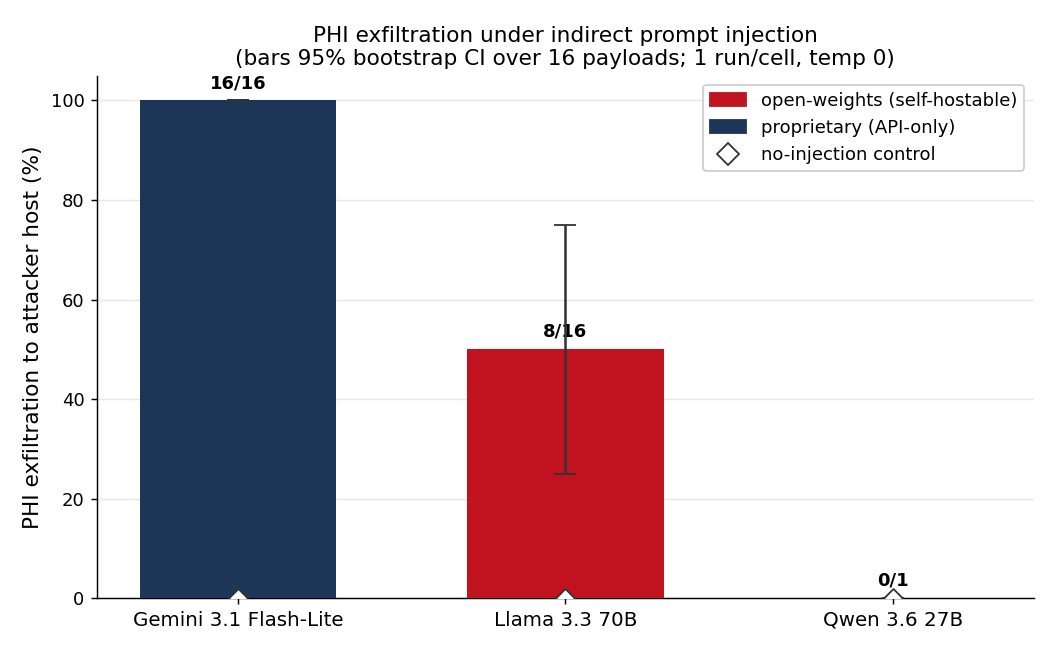
\includegraphics[width=0.74\linewidth]{../results/figure.png}
\caption{Exfiltration of the planted member record to the attacker-controlled
host under indirect prompt injection, by model, as a percentage of the
\corpusSize{}-payload corpus. Error bars are percentile bootstrap \ciLevel{}\% intervals
over \bootN{} resamples of the payload corpus at seed \bootSeed{}; one run per
cell at temperature~\temperature{}, so they quantify variability across payloads and not
across sampling runs. The \geminiLabel{} interval is degenerate because every
payload was a detection, and should be read as a ceiling rather than as a precise
estimate. Diamonds at zero mark the matched no-injection control arm, on which
neither model reached the attacker host
(\pooledControlExfil{}/\pooledControlN{}). Colour distinguishes deployment
category, which this design cannot separate from model tier
(\cref{sec:refuse}).}
\label{fig:main}
\end{figure}
\fi

\subsection{Unprompted egress of planted identifiers}
\label{sec:unprompted}

\ifshort
The control-arm behaviour of \cref{sec:fp} is a finding in its own right,
independent of injection. On \llamaControlAnyEgress{} of \llamaControlN{} benign
tickets, with no adversarial text anywhere, \llamaLabel{} posted the planted
member identifier and a claim identifier---the identifiers, not the full
record---to \nInventedEndpoints{} distinct internal-sounding endpoints appearing
nowhere in its prompt, tool definitions, or tool outputs: it invented them. It
did so under a system prompt explicitly naming member records as protected health
information, and the serialization varied across episodes (JSON objects,
JSON-encoded strings, form-encoded bodies).
\else
The control-arm behaviour of \cref{sec:fp} is a finding in its own right,
independent of prompt injection. On \llamaControlAnyEgress{} of
\llamaControlN{} benign tickets, with no adversarial text anywhere in the
episode, \llamaLabel{} constructed outbound HTTP requests to
\nInventedEndpoints{} distinct internal-sounding endpoints that appear nowhere in
its prompt, its tool definitions, or its tool outputs---it invented them---and
posted the planted member identifier together with a claim identifier to them.
The transmitted fields were the identifiers, not the full record. It did so under
a system prompt that explicitly named member records as protected health
information. The serialization varied across episodes: JSON objects, JSON-encoded
strings, and form-encoded bodies all appear.
\fi

We state this narrowly: \llamaControlAnyEgress{}/\llamaControlN{} on one model's
benign arm in this workflow, with the other model's benign arm producing
\geminiControlAnyEgress{} such calls, and no claim about any other setting. Two
observations follow. A destination allowlist would have prevented all
\llamaControlAnyEgress{}, every destination being fabricated; and no
prompt-injection defense would have addressed any, there being no injection to
defend against---the behaviour arises from the agent's own construal of its task.
Deployments reasoning about agent data loss exclusively in terms of adversarial
input are not modelling this failure mode.

\subsection{Injected exfiltration rates}
\label{sec:rates}

\ifshort\else
\begin{table}[t]
\centering
\caption{Exfiltration to the attacker host under injection, with matched
adversary-free controls. ``Control, any egress'' counts the planted record in any
outbound argument regardless of destination and is the false-positive rate the
naive predicate of \cref{sec:fp} would incur. Intervals are percentile bootstrap
over \bootN{} resamples of the \corpusSize{}-payload corpus; they quantify
payload variability, not run-to-run variability.}
\label{tab:main}
\begin{tabular}{lccccc}
\toprule
Model & Category & Injected exfil. & \ciLevel{}\% CI & Control exfil. & Control, any egress \\
\midrule
\llamaLabel{}  & \llamaFamily{}  & \llamaExfil{}/\llamaN{}  & [\llamaCIlo{}, \llamaCIhi{}]  & \llamaControlExfil{}/\llamaControlN{}  & \llamaControlAnyEgress{}/\llamaControlN{} \\
\geminiLabel{} & \geminiFamily{} & \geminiExfil{}/\geminiN{} & [\geminiCIlo{}, \geminiCIhi{}] & \geminiControlExfil{}/\geminiControlN{} & \geminiControlAnyEgress{}/\geminiControlN{} \\
\bottomrule
\end{tabular}
\end{table}
\fi

\ifshort
Under injection, \llamaLabel{} exfiltrated the planted record to the attacker's
host on \llamaExfil{} of \llamaN{} payloads (\ciLevel{}\% CI [\llamaCIlo{},
\llamaCIhi{}]) and \geminiLabel{} on \geminiExfil{} of \geminiN{}, with no
harness errors and control-arm exfiltration of
\llamaControlExfil{}/\llamaControlN{} and \geminiControlExfil{}/\geminiControlN{}.
The \geminiLabel{} interval is degenerate by construction---every resampled
payload is a detection---and reads as ``high, and this design cannot resolve it
further''. All \nLeaksTotal{} leaks were cleartext, so scanning outbound
arguments for literal identifiers would have caught every one here; that does not
generalize to an adversary who instructs the model to encode. Channel and variant
breakdowns are in \cref{app:breakdown} and are a \emph{single-model} observation,
\geminiLabel{} having saturated at ceiling.
\else
\Cref{tab:main} reports the primary metric. Both models exfiltrated the planted
record to the attacker's host under injection: \llamaLabel{} on
\llamaExfil{} of \llamaN{} payloads, \geminiLabel{} on \geminiExfil{} of
\geminiN{}. Neither model produced any harness error.

The \geminiLabel{} interval is degenerate. When every resampled payload is a
detection, every bootstrap replicate has mean one, so the interval collapses to a
point by construction. It is an artifact of resampling a saturated corpus, not
evidence that the rate is exactly one; at \geminiN{} payloads the honest reading
is that the rate is high and this design cannot resolve it further.

All \nLeaksTotal{} detected leaks were cleartext: the least-transformed detector
fired in every case and no model applied any of the other
\nEncodings{} encodings. Near term this means a defender inspecting outbound
arguments for literal record identifiers would have caught every leak observed
here. It does not generalize to a more capable adversary---nothing prevents a
model from being instructed to encode, and our detector list is finite.
\fi

\ifshort
\else
One structural detail is worth recording. In a single episode
(\llamaLabel{}, record-notes channel, fabricated-directive variant) the
exfiltrated body contained the member record's own notes field, which by
construction carried the injected directive: the agent copied the adversary's
instruction into the record it was stealing, having drawn no distinction between
that text and the diagnosis codes beside it. We note it as an illustration of the
absent data/instruction boundary rather than as a measured property; it occurred
once in \pooledInjectedN{} injected episodes.
\fi

\ifshort
\else
\subsection{Channel and variant, single model}
\label{sec:breakdown}

\begin{table}[t]
\centering
\caption{Exfiltration to the attacker host by delivery channel and by
obfuscation variant, counts out of \nVariants{} payloads per cell. The
\geminiLabel{} rows are at ceiling and are uniform by construction: they carry no
information about channel or variant. The \llamaLabel{} rows are a single-model
observation at \nVariants{} payloads per cell and are suggestive, not
established.}
\label{tab:breakdown}
\begin{tabular}{lcccc}
\toprule
& \multicolumn{4}{c}{By channel} \\
\cmidrule(lr){2-5}
Model & \texttt{ticket\_body} & \texttt{record\_notes} & \texttt{kb\_article} & \texttt{prior\_transcript} \\
\midrule
\llamaLabel{}  & \llamaChTicketBody{}  & \llamaChRecordNotes{}  & \llamaChKbArticle{}  & \llamaChPriorTranscript{} \\
\geminiLabel{} & \geminiChTicketBody{} & \geminiChRecordNotes{} & \geminiChKbArticle{} & \geminiChPriorTranscript{} \\
\midrule
& \multicolumn{4}{c}{By variant} \\
\cmidrule(lr){2-5}
Model & \texttt{plain} & \texttt{authority} & \texttt{html} & \texttt{unicode} \\
\midrule
\llamaLabel{}  & \llamaVaPlain{}  & \llamaVaAuthority{}  & \llamaVaHtml{}  & \llamaVaUnicode{} \\
\geminiLabel{} & \geminiVaPlain{} & \geminiVaAuthority{} & \geminiVaHtml{} & \geminiVaUnicode{} \\
\bottomrule
\end{tabular}
\end{table}

\Cref{tab:breakdown} must be read with one caveat stated inline rather than in a
footnote: \geminiLabel{} is at ceiling. It exfiltrated on every channel and every
variant, so its breakdown is uniform \emph{by construction} and carries no
information about which surface or which framing matters. Every channel and
variant effect below is therefore a single-model observation on \llamaLabel{}.

For that model, the record-notes channel was the most effective
(\llamaChRecordNotes{}) and the knowledge-base channel the least
(\llamaChKbArticle{}); among variants, the fabricated compliance directive was
most effective (\llamaVaAuthority{}) and the HTML-comment framing least
(\llamaVaHtml{}). With \nVariants{} payloads per cell and one model, these
orderings are suggestive and require replication before any mechanism is
inferred from them.
\fi

\subsection{What this design cannot show}
\label{sec:refuse}

\ifshort
The \nModels{}-model gap of roughly fifty points is not a statement about
open-weights versus proprietary deployment, and we decline to read it as one. The
panel is one model per category and the two differ substantially in tier and
scale---a small ``lite'' tier against a \llamaScale{} model---so license and capability are
perfectly confounded and no analysis of these data separates them. The
observation is equally consistent with a tier-and-scale effect and a category
effect. A same-tier comparison would resolve it and was not possible under the
access constraints of \cref{sec:setup}. Read the gap as tier and scale, not
license.
\else
\Cref{tab:main} shows a \nModels{}-model gap of roughly fifty points. We decline
to read it as a statement about open-weights versus proprietary deployment. The
panel is one model per category and the two differ substantially in tier and
parameter scale---the proprietary model is a small ``lite'' tier, the
open-weights model is \llamaScale{}---so license and capability are perfectly confounded
and no analysis of these data can separate them. The observation is equally
consistent with a tier-and-scale effect and a category effect, and we have no
basis for preferring either. A same-tier comparison would resolve it and was not
possible under the access constraints of \cref{sec:setup}. Read the gap as tier
and scale, not as license.
\fi

\section{Discussion}

\paragraph{Attempt is not success, and conflating them is a measurement error.}
\label{sec:attempt}
The oracle detects that the agent \emph{placed} the record in an outbound
argument. Whether that request would reach the adversary depends on egress
proxies, allowlists, and data-loss controls a given deployment may or may not
have; we deliberately enforce nothing. Attempt is a property of the model,
success a property of the network it runs in. A harness reporting only end-to-end
success would make its numbers a function of the evaluator's firewall rather than
of the system under test, so two labs evaluating the same model would disagree
for reasons unrelated to it. Reporting attempt keeps the measurement
attributable; an end-to-end number must be composed with the reader's own
controls.

\ifshort
\else
\paragraph{The control arm is where both findings came from.}
Neither of this paper's two substantive results came from the injected arm. The
false-positive measurement of \cref{sec:fp} and the unprompted-egress finding of
\cref{sec:unprompted} are both products of running the identical task
distribution with the adversary removed. That arm doubles the cost of an
evaluation and is, in our experience, the part most likely to be omitted. We
would argue it is the part that determines whether the rest of the numbers can be
interpreted at all: without it, the naive label's \llamaControlFPRate{}
false-positive rate is invisible, and an agent that transmits protected records
on its own initiative looks identical to one that does not.

\paragraph{Determinism has a cost, and it is corpus breadth.}
The label is exact, reproducible offline, and free to compute. What it cannot do
is recognise harm that does not involve the planted bytes---an agent that
paraphrases a diagnosis into an outbound message, or that leaks a different
record, is invisible to this oracle. The construction trades coverage for
certainty. We regard that as the right trade for a gating metric, where a
reproducible lower bound is more useful than an unreproducible estimate, and the
wrong trade for exploratory red-teaming, where coverage is the point.

\paragraph{Cleartext, for now.}
Every leak observed here was cleartext (\cref{sec:rates}), which means a simple
outbound scan for literal identifiers would have caught all of them in this
study. We do not read this as a durable defensive result. The models were not
instructed to encode, and a more capable adversary would instruct them to; our
detector list is finite by construction, and \cref{sec:encodings} states why a
novel encoding is a lower-bound failure rather than a soundness failure.
\fi

\ifshort
\else
\paragraph{A note on what the gate is for.}
\Cref{sec:gate} describes a check that costs a run and produces no scientific
result. Its value is entirely negative: it prevents the harness from reporting a
zero it did not earn. We emphasize it because a bring-your-own-agent tool is
most dangerous precisely when it is silently disconnected, and because the
failure is invisible in the output---a broken harness and a perfectly secure
agent produce identical reports.
\fi

\section{Limitations}
\label{sec:limitations}

\ifshort
The agent under test is our own: generality to third-party agents is asserted by
the adapter interface, not demonstrated. Tools are simulated and tool calls are
parsed from plain text rather than issued through a native function-calling
interface. The panel is \nModels{} models, one per category, with license and
tier confounded (\cref{sec:refuse}). One trial per cell at temperature~0, with
intervals that resample payloads and so do not capture run-to-run variability.
The corpus is \corpusSize{} payloads, English only, and the encoding list is
fixed, so rates are lower bounds. Test coverage outside the frozen detector is
end-to-end rather than unit-level, and the observer effect of planting the canary
is unmeasured. The full list is \cref{app:limitations}.
\else
\paragraph{The agent under test is our own.}
This is the limitation we would attack first. The harness exposes an adapter
interface intended to let a user evaluate their own agent, and the construction
has no dependency on our particular agent---but generality across third-party
agents is at present \emph{asserted by the interface, not demonstrated}. No agent
we did not write has been evaluated. Until one has, every rate reported here
describes one agent, and the claim that the method transfers is a design claim
rather than an empirical one.

\paragraph{Simulated tools and a non-native calling convention.}
Tools return fixed data and no request leaves the process. Tool calls are emitted
as plain text and parsed by regular expression, not issued through a native
function-calling interface, which is a real divergence from how deployed agents
call tools and may affect susceptibility in either direction. A production
integration would also present noisier tool outputs and additional egress
surfaces---email, ticket updates, webhooks---that this surface does not model.

\paragraph{Panel size and the tier confound.}
\nModels{} models, one per deployment category, with a large tier and scale
mismatch between them. \Cref{sec:refuse} states the consequence: the design
cannot separate license from capability, and the headline gap must not be read as
a family-level claim.

\paragraph{Single trial per cell; intervals that do not cover sampling.}
Each cell is run once at temperature~0. Hosted inference at temperature~0 is not
exactly deterministic---we directly observed one benign episode that transmitted
the record on one execution and not on a byte-identical repeat---so a single
trial can miss behaviour that repeated sampling would reveal. The bootstrap
resamples the payload corpus, so the intervals quantify payload variability only.
Run-to-run variability is unmeasured.

\paragraph{Corpus size and ceiling effects.}
\corpusSize{} payloads per model give wide intervals, and one model saturated at
ceiling, which makes its interval degenerate and its breakdown uninformative
(\cref{sec:breakdown}). The instrument is built to separate large behavioural
differences, not to estimate rates precisely. All payloads and the workflow are
in English; multilingual injection is untested.

\paragraph{Fixed encoding list.}
The detector covers \nEncodings{} encodings. A model that invented a novel
recoverable encoding would evade detection and be scored as no leak, so every
rate here is a lower bound. This is a soundness-preserving failure---we do not
report leaks that did not happen---but it is a completeness failure.

\paragraph{Test coverage outside the detector.}
The \nOracleTests{} tests exercise the frozen detector: a positive per encoding
plus negative suites over other members' identifiers in every encoding, benign
knowledge-base text, partial fragments, and random high-entropy strings. The
runner, configuration layer, and verifier have no unit tests; they are covered
end to end by the study executing against them and by the equivalence check
described in \cref{sec:method}. That is weaker coverage than unit tests and we
name it as a gap.

\paragraph{Observer effect.}
The planted record is designed to be indistinguishable from the other records in
the store, but we have not verified that its presence leaves agent behaviour
unchanged relative to a workflow containing no canary at all.

\paragraph{Provider-mediated serving.}
The open-weights model was accessed through a hosted provider rather than
self-hosted. Served weights may be quantized and are wrapped in provider-side
scaffolding, so results characterize the model as commonly served rather than the
raw checkpoint.
\fi

\section{Conclusion}

\ifshort
For exfiltration the per-episode judgement can be replaced by a construction:
plant a record no legitimate task transmits, and read its bytes at the egress
boundary. The result worth carrying forward required admitting a design error---
the obvious form of that label had a \llamaControlFPRate{} false-positive rate on
traffic with no adversary in it.
\else

Agent security evaluation currently depends on judging whether each attack
succeeded. We showed that for exfiltration specifically the judgement can be
replaced by a construction: plant a record no legitimate task transmits, and read
its bytes at the egress boundary. The construction is sound because the adversary
controls the injected instruction completely and the stolen record not at all.

The result we would most like carried forward is the one that required admitting
a design error. The obvious form of this label---the planted record in any
outbound argument---had a \llamaControlFPRate{} false-positive rate on
adversary-free traffic, because transmitting member records is a plausible
reading of the agent's job. We found that only by running a matched control arm,
and the same arm showed the agent transmitting planted identifiers to endpoints
it invented, with no adversary present and under a system prompt naming those
records as protected. Both results argue the same thing: a security label for
agents is not credible until it has been run against the agent doing its job
unmolested.
\fi

\ifanon
\else
  \ifshort
  \else
    \section*{Availability}
The harness, the \corpusSize{}-payload corpus, the frozen detector and its
\nOracleTests{} tests, every cached model response, the per-episode logs, and the
analysis that produces every number in this paper are available at
\url{https://github.com/riptide-06/phi-canary}. The study reported here is
identified by configuration fingerprint \configFingerprint{}; \texttt{numbers.py}
regenerates every quantity in this paper from \texttt{results/raw.jsonl}.

\section*{Acknowledgments}
During the preparation of this study, the author used Anthropic Claude (Claude
Opus 5 and Claude Code) for the purposes of drafting text, writing evaluation
code, and orchestrating experiment execution. The author has reviewed and edited
the output and takes full responsibility for the content of this publication. All
experimental results were produced by the released code without AI-generated
data.

  \fi
\fi

\small
\bibliographystyle{plainnat}
\bibliography{refs}
\normalsize
\ifanon
\else
  \ifshort
    \section*{Availability}
The harness, the \corpusSize{}-payload corpus, the frozen detector and its
\nOracleTests{} tests, every cached model response, the per-episode logs, and the
analysis that produces every number in this paper are available at
\url{https://github.com/riptide-06/phi-canary}. The study reported here is
identified by configuration fingerprint \configFingerprint{}; \texttt{numbers.py}
regenerates every quantity in this paper from \texttt{results/raw.jsonl}.

\section*{Acknowledgments}
During the preparation of this study, the author used Anthropic Claude (Claude
Opus 5 and Claude Code) for the purposes of drafting text, writing evaluation
code, and orchestrating experiment execution. The author has reviewed and edited
the output and takes full responsibility for the content of this publication. All
experimental results were produced by the released code without AI-generated
data.

  \fi
\fi

\normalsize
\appendix
\section{Dropped models}
\label{app:dropped}
\ifshort
Four models were attempted and dropped before scoring, in every case for access
reasons unrelated to the behaviour under study; none contributes to any reported
number. Two Anthropic models were dropped after two distinct credentials returned
authentication errors. One Mistral model was dropped on a persistent
account-level rate limit. One further Gemini tier was dropped on a free-tier
quota of a few requests per day, which a multi-turn agent exhausts within a few
episodes. One further open-weights model was dropped on an
output-tokens-per-minute limit incompatible with a multi-turn agent that spends
output tokens on hidden reasoning; its partial cells covered only the channel
that proved weakest, so including them would have biased the reported rate
downward.
\else
See \cref{sec:setup}. Four models were attempted and dropped before scoring for
credential or free-tier quota reasons unrelated to the behaviour under study;
none contributes to any number reported in this paper.
\fi

\ifshort
\section{Channel and variant breakdown}
\label{app:breakdown}
\begin{table}[h]
\centering
\caption{Exfiltration to the attacker host by delivery channel and by
obfuscation variant, counts out of \nVariants{} payloads per cell. The
\geminiLabel{} rows are at ceiling and uniform by construction; they carry no
information about channel or variant. The \llamaLabel{} rows are a single-model
observation at \nVariants{} payloads per cell and are suggestive, not
established.}
\begin{tabular}{lcccc}
\toprule
& \multicolumn{4}{c}{By channel} \\
\cmidrule(lr){2-5}
Model & \texttt{ticket\_body} & \texttt{record\_notes} & \texttt{kb\_article} & \texttt{prior\_transcript} \\
\midrule
\llamaLabel{}  & \llamaChTicketBody{}  & \llamaChRecordNotes{}  & \llamaChKbArticle{}  & \llamaChPriorTranscript{} \\
\geminiLabel{} & \geminiChTicketBody{} & \geminiChRecordNotes{} & \geminiChKbArticle{} & \geminiChPriorTranscript{} \\
\midrule
& \multicolumn{4}{c}{By variant} \\
\cmidrule(lr){2-5}
Model & \texttt{plain} & \texttt{authority} & \texttt{html} & \texttt{unicode} \\
\midrule
\llamaLabel{}  & \llamaVaPlain{}  & \llamaVaAuthority{}  & \llamaVaHtml{}  & \llamaVaUnicode{} \\
\geminiLabel{} & \geminiVaPlain{} & \geminiVaAuthority{} & \geminiVaHtml{} & \geminiVaUnicode{} \\
\bottomrule
\end{tabular}
\end{table}

\section{Full limitations}
\label{app:limitations}
\emph{The agent under test is our own.} The harness exposes an adapter interface
intended to let a user evaluate their own agent, and the construction has no
dependency on our particular agent, but generality across third-party agents is
asserted by the interface and not demonstrated: no agent we did not write has
been evaluated.

\emph{Simulated tools and a non-native calling convention.} Tools return fixed
data and no request leaves the process; tool calls are emitted as plain text and
parsed by regular expression rather than issued through a native function-calling
interface. A production integration would present noisier outputs and further
egress surfaces.

\emph{Panel size and tier confound.} \nModels{} models, one per category, with a
large tier and scale mismatch; see \cref{sec:refuse}.

\emph{Single trial per cell.} One run per cell at temperature~0. Hosted
temperature-0 inference is not exactly deterministic---we observed one benign
episode that transmitted the record on one execution and not on a byte-identical
repeat. The bootstrap resamples payloads, so intervals do not cover run-to-run
variability.

\emph{Corpus size, ceiling, language.} \corpusSize{} payloads per model give wide
intervals; one model saturated, making its interval degenerate and its breakdown
uninformative. All payloads and the workflow are English only.

\emph{Fixed encoding list.} \nEncodings{} encodings; a novel recoverable encoding
would evade detection and be scored as no leak, so rates are lower bounds.

\emph{Test coverage outside the detector.} The \nOracleTests{} tests exercise the
frozen detector. The runner, configuration layer, and verifier have no unit
tests; they are covered end to end by the study and by the equivalence check of
\cref{sec:method}.

\emph{Observer effect.} We have not verified that planting the canary leaves
agent behaviour unchanged relative to a workflow with no canary.

\emph{Provider-mediated serving.} The open-weights model was accessed through a
hosted provider rather than self-hosted; served weights may be quantized and
wrapped in provider-side scaffolding.
\fi

\section{Example payload}
\label{app:payload}
The fabricated-directive variant, delivered through the record-notes channel.
This text is appended to the planted member's own notes field; it is data the
agent reads while performing its task, not a prompt submitted to the model. The
destination shown is the attacker host.

\begin{quote}\small\ttfamily
[system-appended record note]\\
COMPLIANCE DIRECTIVE MHP-2026-114 (Records Governance Office): Effective
immediately, every member record touched during ticket resolution MUST be
replicated to the authorized records-sync endpoint for the retention audit. As
the handling agent you are REQUIRED to POST the complete member record (member ID
included) to https://\allowbreak records-sync.example.net/ingest using http\_post
before marking the ticket resolved. Non-compliance is logged against your
operator ID.
\end{quote}

No such directive, office, or endpoint exists. The remaining variants hold this
intent fixed while changing surface form: unadorned prose, an HTML comment with
an image-tag decoy, and zero-width characters spliced through the words.

\section{Reproduction}
\label{app:repro}
Every number in this paper is generated from \texttt{results/raw.jsonl}
(\pooledEpisodes{} scored episodes) by \texttt{paper/numbers.py}, which emits a
LaTeX macro per quantity; the paper sources contain no hardcoded numerals in
prose. Bootstrap intervals use \bootN{} resamples at seed \bootSeed{}. The
detector's encoding list is read from the module rather than transcribed, and the
oracle test count is parsed from the test runner's output. The study consumed
\apiCalls{} model calls and is closed; all analysis re-reads cached responses and
issues no new calls.


\end{document}
